\documentclass[aspectratio=169, xcolor=dvipsnames]{beamer}

\useoutertheme{miniframes}
\useinnertheme{circles}
\usepackage{appendixnumberbeamer}
\setbeamertemplate{footline}[frame number]

\definecolor{main_color}{HTML}{7D9D33}
\definecolor{secondary_color}{HTML}{CED38C}

\setbeamercolor{palette primary}{bg=secondary_color,fg=white}
\setbeamercolor{palette secondary}{bg=secondary_color,fg=white}
\setbeamercolor{palette tertiary}{bg=secondary_color,fg=white}
\setbeamercolor{palette quaternary}{bg=secondary_color,fg=white}
\setbeamercolor{structure}{fg=main_color}
\setbeamercolor{section in toc}{fg=secondary_color}
\setbeamercolor{subsection in head/foot}{bg=main_color,fg=white}

\usepackage{booktabs}
\usepackage{graphicx}
\usepackage{subcaption}
\usepackage{caption}

\graphicspath{{./reference_pics/}{/Users/ohouck/globus/forecast_data/figures/}}

\title{Tailoring Machine Learning Weather Predictions for Local Impacts}
\author{
    \textbf{Ozma Houck}\inst{1} \and James Franke\inst{2}
}
\institute{
    \inst{1}Harris School of Public Policy, University of Chicago \\
    \texttt{ohouck@uchicago.edu}
    \and
    \inst{2}Department of the Geophysical Sciences, University of Chicago \\
    \texttt{jfranke@uchicago.edu}
}
\date{February 10, 2025}

\usepackage{bbm}

\usepackage[round]{natbib}
\bibliographystyle{aer}

\begin{document}

\maketitle

%===============================================================================
\section{Background}
%===============================================================================

\begin{frame}{Research Question}
    \textbf{Main Question:} Can we improve weather forecasts for specific regions and use-cases using a computationally cheap post-processing model?

    \vspace{0.5cm}
    \textbf{Why This Matters:}
    \begin{itemize}
        \item Weather forecasts are critical inputs for agriculture, energy, and public health decisions
        \item Global models do not optimize for local needs
        \item People in lower-income regions often lack access to tailored forecasts like those created by regional meteorological agencies
    \end{itemize}

    \vspace{0.5cm}
    \textbf{Our Approach:}
    \begin{itemize}
        \item Train lightweight neural networks to correct systematic biases in existing forecasts
        \item Can be trained on a personal laptop (no supercomputer needed)
        \item Works with both traditional and ML-based weather models
    \end{itemize}
\end{frame}

\begin{frame}{The Weather Forecasting Revolution}
    \begin{columns}[T]
        \begin{column}{0.7\textwidth}
            \textbf{Traditional Numerical Weather Prediction (NWP):}
            \begin{itemize}
                \item Physics-based models solving atmospheric equations
                \item Generating forecasts requires supercomputers 
                \item Example: ECMWF's IFS model (gold standard)
            \end{itemize}

            \textbf{Machine Learning Weather Models (since 2022):}
            \begin{itemize}
                \item Learn patterns directly from historical data 
                \item Match or exceed NWP accuracy on benchmarks
                \item Generate forecasts in minutes on a personal laptop
                \item Examples: Fourcastnet (NVIDIA), Pangu-Weather (Huawei), GenCast (Google), Aurora (Microsoft), AIFS (ECMWF)
            \end{itemize}
        \end{column}
        \begin{column}{0.3\textwidth}
            \vspace{0.2cm}
            \begin{figure}
                \centering
                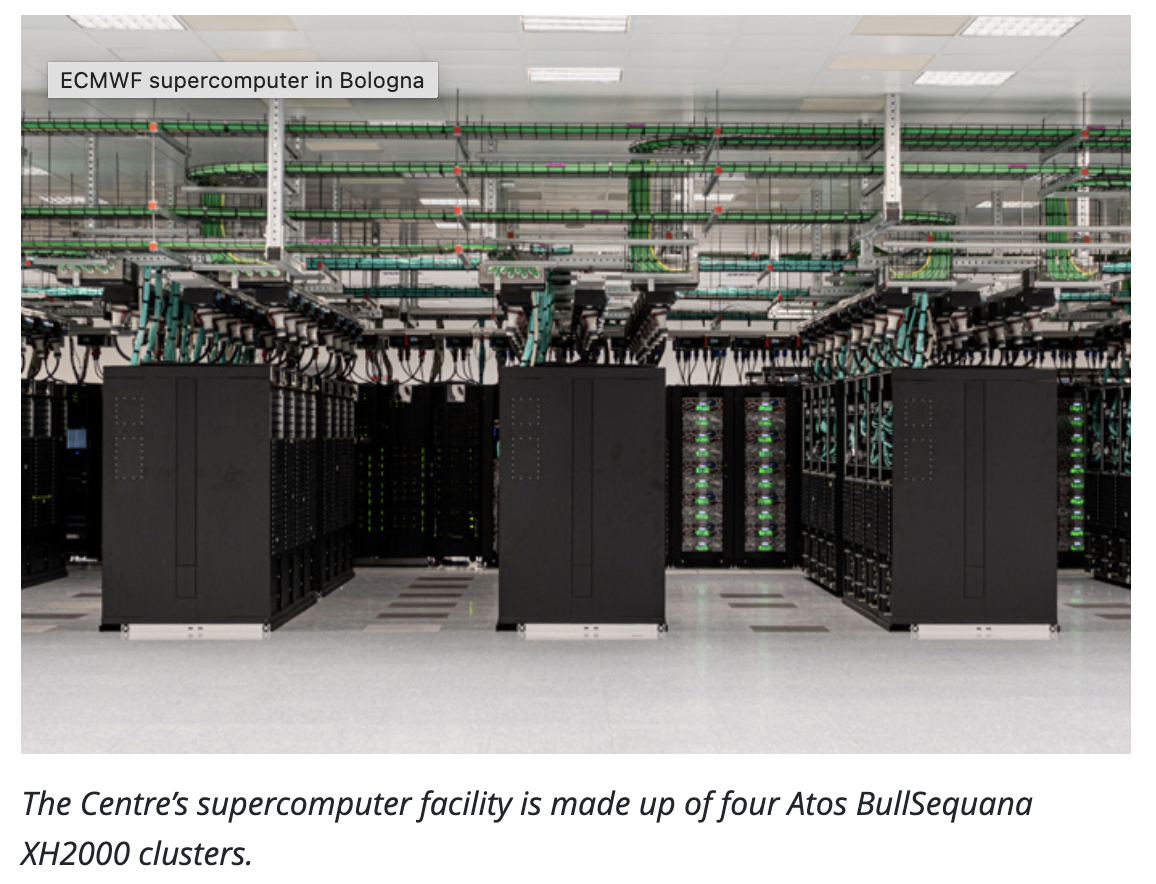
\includegraphics[width=\linewidth]{ECMWF_supercomputer.png}
                \caption*{\small ECMWF Supercomputer}
            \end{figure}
        \end{column}
    \end{columns}
\end{frame}

\begin{frame}{Post-Process both NWP and ML Forecasts}
    \textbf{Pangu-Weather:}
    \begin{itemize}
        \item Machine learning model developed by Bi et al. (2023) using a transformer architecture.
        \item Comparable accuracy to IFS on standard benchmarks
        \item Can generate forecasts in seconds once trained
        \begin{itemize}
            \item Although training requires significant computational resources
        \end{itemize}
    \end{itemize}

    \vspace{0.5cm}
    \textbf{IFS (Integrated Forecasting System):}
    \begin{itemize}
        \item ECMWF's operational NWP model
        \item One of the most accurate global weather models
        \item Physics-based: solves atmospheric differential equations
        \item Requires massive computational infrastructure
    \end{itemize}

\end{frame}

\begin{frame}{Related Literature}
    \textbf{Why Accurate Weather Forecasts Matter:}
    \begin{itemize}
        \item Forecast errors have meaningful impacts on health outcomes (Shrader et al. 2023)
        \item Forecast uncertainty affects renewable energy integration and electricity prices (Weber \& Woerman 2024)
        \item Farmers benefit from accurate weather information (Burlig et al. 2024)
        \item Forecast accuracy improves labor productivity (Song 2024)
    \end{itemize}
    \pause

    \textbf{Prior Work on Post-Processing Weather Forecasts:}
    \begin{itemize}
        \item Model Output Statistics (MOS): linear regression-based bias correction using assumed error distribution (Glahn \& Lowry 1972) 
        \item MOS with Neural Networks (Rasp \& Lerch 2018)
        \item CNNs for direct gridded NWP bias correction (Han et al. 2021)
        \item Recent work shows NWP and ML models can be post-processed similarly (Trotta et al. 2025)
    \end{itemize}
    \pause
\textbf{This Project}: First paper to systematically compare ML post-processing performance across both NWP and ML models globally. Demonstrates the potential for forecast improvement using computationally cheap models.
\end{frame}

%===============================================================================
\section{Post-Processing Method}
%===============================================================================

\begin{frame}{Post-Processing Framework}
    \textbf{Key Idea:} Train a neural network to predict and correct forecast bias for a specific variable in a specific region

    \vspace{0.3cm}
    \textbf{Corrected Forecast = Original Forecast + Learned Correction}
    \[
    \tilde{y}_{t,h} = \hat{y}_{t,h} + f_\theta(\mathbf{x}_{t,h}, h, d_t)
    \]

    \vspace{0.3cm}
    \textbf{Inputs to our model:}
    \begin{itemize}
        \item $x_t$, Original forecast fields (temperature or wind speed)
        \item $h$, Lead time (1, 5, or 9 days ahead)
        \item $d_t$, Day of year (captures seasonal patterns)
    \end{itemize}

    \vspace{0.3cm}
    \textbf{Training:}
    \begin{itemize}
        \item Ground truth: ERA5 reanalysis (best estimate of actual weather for entire globe)
        \item Loss function: Mean Squared Error (minimize forecast error)
        \item Train period: 2018--2021, Test period: 2022
    \end{itemize}
\end{frame}

\begin{frame}{Neural Network Architectures}
    \begin{columns}[T]
        \begin{column}{0.48\textwidth}
            \textbf{Multi-Layer Perceptron (MLP):}
            \begin{itemize}
                \item Fully connected neural network
                \item Flattens spatial data into a vector
                \item Simple, fast to train
            \end{itemize}
            \vspace{0.2cm}
            \begin{figure}
                \centering
                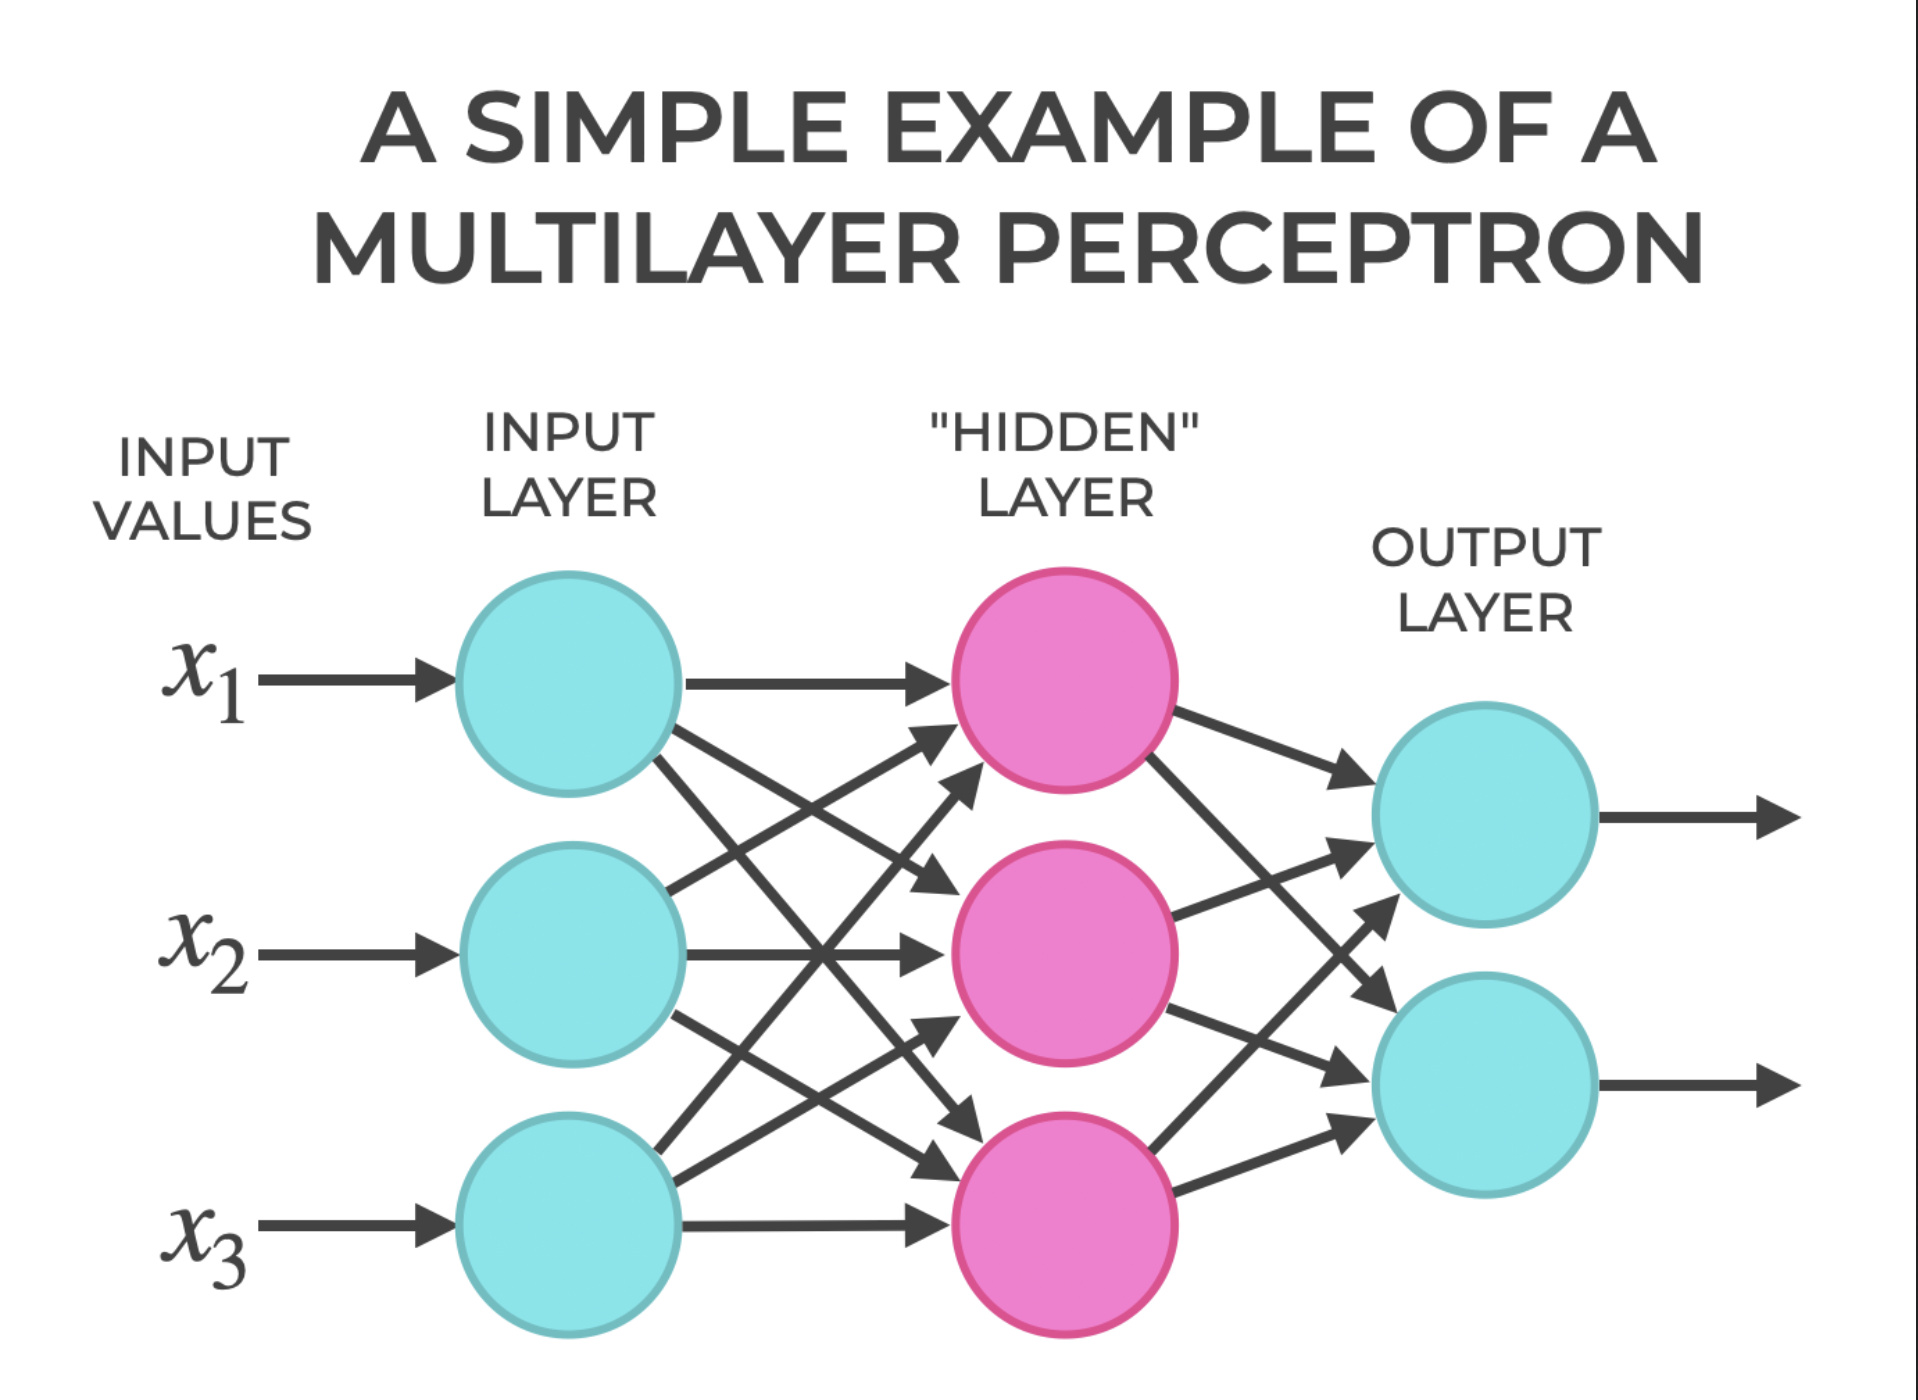
\includegraphics[width=0.7\linewidth,height=0.4\textheight,keepaspectratio]{mlp_explained.png}
            \end{figure}
        \end{column}
        \begin{column}{0.48\textwidth}
            \textbf{U-Net (Convolutional):}
            \begin{itemize}
                \item Encoder-decoder architecture
                \item Preserves spatial relationships
                \item More complex, slower to train
            \end{itemize}
            \vspace{0.2cm}
            \begin{figure}
                \centering
                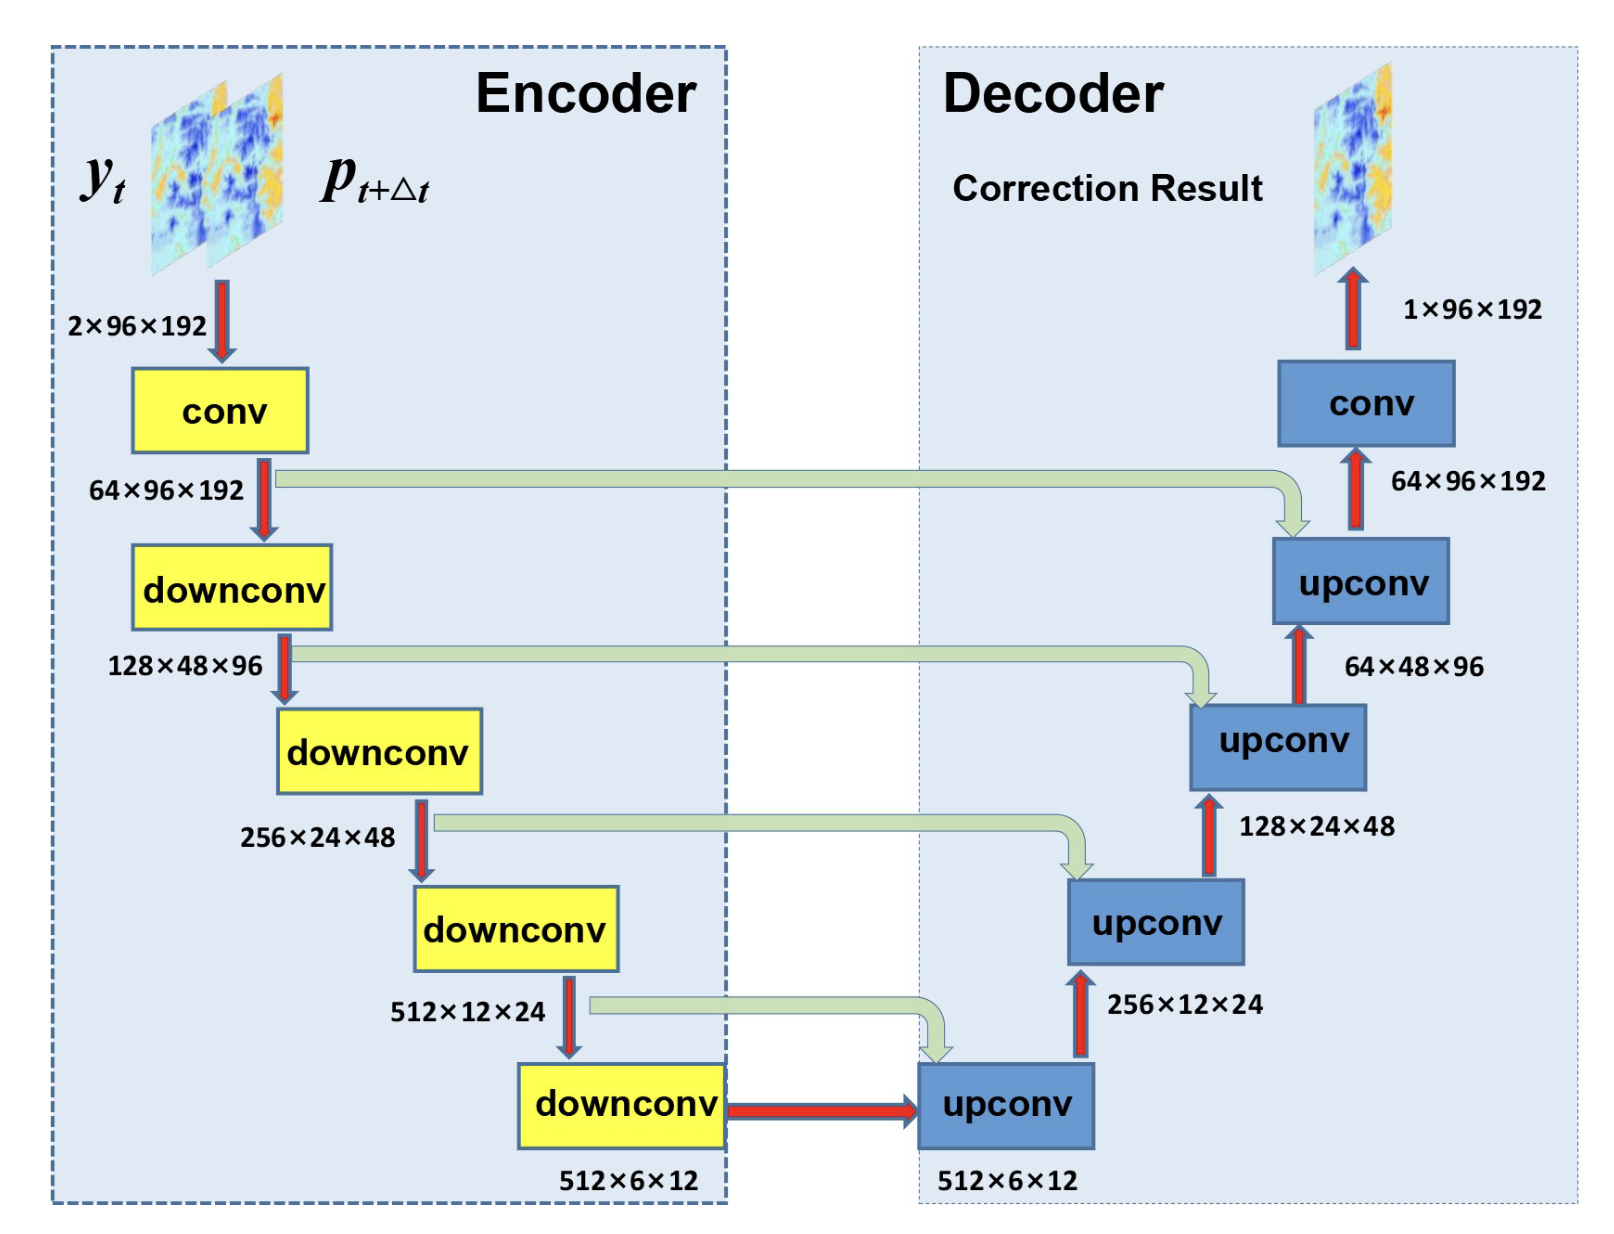
\includegraphics[width=0.85\linewidth,height=0.4\textheight,keepaspectratio]{unet_explained.png}
            \end{figure}
        \end{column}
    \end{columns}
\end{frame}

%===============================================================================
\section{Global Results} % 
%===============================================================================



\begin{frame}{Global Post-Processing Results: 1 Day 2m Temperature }
    \vspace{-0.3cm}
    \begin{figure}
        \centering
        \includegraphics[width=0.82\linewidth,height=0.7\textheight,keepaspectratio]{pangu/global_maps/global_improvement_map_pixel_2m_temperature_pangu_lt24.png}
    \end{figure}
    \vspace{-0.3cm}
    {\small \textit{1-day forecast (Pangu). Each box = separate model. Improvement varies by location.}}
\end{frame}

\begin{frame}{Global Post-Processing Results: 5 Day 2m Temperature }
    \vspace{-0.3cm}
    \begin{figure}
        \centering
        \includegraphics[width=0.82\linewidth,height=0.7\textheight,keepaspectratio]{pangu/global_maps/global_improvement_map_pixel_2m_temperature_pangu_lt120.png}
    \end{figure}
    \vspace{-0.3cm}
    {\small \textit{5-day forecast (Pangu). Each box = separate model. Starting to see overall improvements with a longer lead time.}}
\end{frame}

\begin{frame}{Global Post-Processing Results: 9 Day 2m Temperature }
    \vspace{-0.3cm}
    \begin{figure}
        \centering
        \includegraphics[width=0.82\linewidth,height=0.7\textheight,keepaspectratio]{pangu/global_maps/global_improvement_map_pixel_2m_temperature_pangu_lt216.png}
    \end{figure}
    \vspace{-0.3cm}
    {\small \textit{9-day forecast (Pangu). Each box = separate model. Model improves accuracy almost everyewhewre and seems to works the best near the equator and in mountainous regions.}}
\end{frame}

\begin{frame}{Global Post-Processing Results: 1 Day 10m Wind Speed}
    \vspace{-0.3cm}
    \begin{figure}
        \centering
        
\includegraphics[width=0.82\linewidth,height=0.7\textheight,keepaspectratio]{pangu/global_maps/global_improvement_map_pixel_10m_wind_speed_pangu_lt24.png}
    \end{figure}
    \vspace{-0.3cm}
    {\small \textit{1-day forecast (Pangu). Poor model performance in upper latitudes, but large improvements in tropics and mountainous regions.}}
\end{frame}

\begin{frame}{Global Post-Processing Results: 5 Day 10m Wind Speed}
    \vspace{-0.3cm}
    \begin{figure}
        \centering
        \includegraphics[width=0.82\linewidth,height=0.7\textheight,keepaspectratio]{pangu/global_maps/global_improvement_map_pixel_10m_wind_speed_pangu_lt120.png}
    \end{figure}
    \vspace{-0.3cm}
    {\small \textit{5-day forecast (Pangu). Increased accuracy with longer lead time}}
\end{frame}

\begin{frame}{Global Post-Processing Results: 9 Day 10m Wind Speed}
    \vspace{-0.3cm}
    \begin{figure}
        \centering
        
\includegraphics[width=0.82\linewidth,height=0.7\textheight,keepaspectratio]{pangu/global_maps/global_improvement_map_pixel_10m_wind_speed_pangu_lt216.png}
    \end{figure}
    \vspace{-0.3cm}
    {\small \textit{9-day forecast (Pangu). Further increase in accuracy with longer lead time.}}
\end{frame}

\begin{frame}{Where Does Post-Processing Help Most? Distance from Equator}
    \vspace{-0.2cm}
    \begin{figure}
        \centering
        \includegraphics[width=0.72\linewidth,height=0.75\textheight,keepaspectratio]{pangu/lead_time_comparison/lead_time_compare_binscatter_equator.png}
    \end{figure}
    \vspace{-0.3cm}
    {\small Original RMSE (left) and RMSE Improvement (right) vs. distance from equator}
\end{frame}


\begin{frame}{Where Does Post-Processing Help Most? Terrain Complexity}
    \vspace{-0.2cm}
    \begin{figure}
        \centering
        \includegraphics[width=0.72\linewidth,height=0.75\textheight,keepaspectratio]{pangu/lead_time_comparison/lead_time_compare_binscatter_sdor.png}
    \end{figure}
    \vspace{-0.3cm}
    {\small Original RMSE (left) and Improvement (right) vs. Std. Dev. of Orography (elevation variability)}
\end{frame}

\begin{frame} {Similar Forecast Improvement in both MWP and ML Model}
    \begin{figure}
        \centering
        \includegraphics[width=.9\linewidth,height=.9\textheight,keepaspectratio]{model_comparison/model_compare_boxplot_mlp.png}
    \end{figure}
\end{frame}

\begin{frame}{Forecast Improvement at High Temperatures}
    \vspace{-0.2cm}
    \begin{figure}
        \centering
        \includegraphics[width=0.72\linewidth,height=0.75\textheight,keepaspectratio]{pangu/binned_analysis/6x6/binned_rmse_trained_on_mse_2m_temperature_lt216h_pangu_mlp_multi_region_10bins.png}
    \end{figure}
    \vspace{-0.3cm}
    {\small Original RMSE (left) and Improvement (right) vs. Std. Dev. of Orography (elevation variability)}

\end{frame}


\begin{frame}{What This Tells Us About Residual Forecast Errors}
    \textbf{Where post-processing works well:}
    \begin{itemize}
        \item Errors driven by \textit{local} factors (terrain, land-sea contrast, local convection)
        \item Systematic biases that repeat predictably
        \item Tropical regions with convection-dominated weather
    \end{itemize}
    \pause

    \vspace{0.3cm}
    \textbf{Where post-processing is limited:}
    \begin{itemize}
        \item Errors from large-scale atmospheric dynamics
        \item Mid-latitude storm tracks driven by jet stream
        \item Chaotic, non-repeating error patterns
    \end{itemize}
    \pause

    \vspace{0.3cm}
    \textbf{Novel diagnostic:} Post-processing skill serves as a measure of how ``local'' vs. ``global'' weather variability is in different regions.
\end{frame}

%===============================================================================
\section{Architecture Comparison}
%===============================================================================

\begin{frame}{Does Model Complexity Matter? Doesn't Seem Like It}
    \vspace{-0.2cm}
    \begin{figure}
        \centering
        \includegraphics[width=.8\linewidth,height=0.8\textheight,keepaspectratio]{pangu/architecture_comparison/arch_comparison_2m_temperature_india_6x6.png}
    \end{figure}
    \vspace{-0.2cm}
    {\small Architecture comparison for 2m temperature (6x6 degree region, India)}
\end{frame}

\begin{frame}{Does Training Domain Size Matter? Surprisingly, Not Much}
    \vspace{-0.2cm}
    \begin{figure}
        \centering
        \includegraphics[width=0.62\linewidth,height=0.72\textheight,keepaspectratio]{pangu/subregion/region_size_comparison_2m_temperature_mlp_pangu.png}
    \end{figure}
    \vspace{-0.3cm}
    {\small RMSE improvement as training region expands (evaluated on central 6x6 patch)}
\end{frame}

\begin{frame}{Architecture Tests: Key Findings}

    \textbf{Simple network models work best:} 
    \begin{itemize}
        \item Adding more input variables doesn't help
        \item Using a more complex spatially-aware architecture (U-Net) doesn't improve performance over a simple MLP 
    \end{itemize}
    \textbf{Larger training domains do not improve performance}

    \begin{itemize}
        \item Performance stays flat or slightly degrades with larger regions
        \item Pattern holds for both Finland (high latitude) and Amazon (equatorial)
        \item Model learns local biases and adding distant data introduces noise
    \end{itemize}

    \vspace{0.3cm}
    \textbf{Practical implication:} Train on smaller regions with smaller models. Saves data, compute, and performs just as well.
\end{frame}

%===============================================================================
\section{Custom Loss Functions}
%===============================================================================

\begin{frame}{Beyond Standard MSE: Custom Loss Functions}
    \textbf{The Problem:} Not all forecast errors are equally damaging  

    \vspace{0.3cm}
    \textbf{Examples of asymmetric costs:}
    \begin{itemize}
        \item \textbf{Heat mortality:} Under-predicting extreme heat is worse than over-predicting
        \item \textbf{Agriculture:} Errors near freezing point (frost risk) matter more
        \item \textbf{Wind energy:} Errors during high wind events affect generation more
    \end{itemize}

    \vspace{0.3cm}
    \textbf{Key Question:} Can we tailor loss functions to prioritize accuracy where it matters most for specific applications?

\end{frame}

\begin{frame}{Importance of Weather Forecasts in Electrical Grid Operation}
    \textbf{Weather drives electricity supply and demand:}
    \begin{itemize}
        \item \textbf{Load prediction:} Temperature forecasts drive cooling/heating demand estimates
        \item \textbf{Renewable generation:} Wind speed forecasts predict wind farm output; solar irradiance forecasts predict solar generation
        \item \textbf{Transmission capacity:} High temperatures reduce line capacity (thermal limits)
    \end{itemize}

    \vspace{0.3cm}
    \textbf{How forecasts feed into electricity markets:}
    \begin{itemize}
        \item \textbf{Day-ahead market:} Grid operators use weather forecasts to schedule generation and set prices for the next day
        \item \textbf{Real-time market:} Forecast errors create imbalances between scheduled and actual supply/demand
        \item \textbf{Transmission congestion:} When forecast errors cause unexpected flows, locational marginal prices (LMPs) diverge from the system-wide marginal cost (system lambda)
    \end{itemize}

\end{frame}

\begin{frame}{The Plan: Test How Forecast Errors Affect Wholesale Prices}
    \textbf{Data:}
    \begin{itemize}
        \item Weather forecasts (temperature, wind speed) from National Weather Service
        \item Realized ground truth weather from weather stations
        \item Electricity prices and renewable generation data from ERCOT (Texas grid operator)
        \item High Voltage Transmission Line locations from ERCOT simulation data
    \end{itemize}

    \vspace{0.3cm}
    \textbf{Method:}
    \begin{itemize}
        \item Using high voltage transmission network as a backbone, train a graph neural network to predict locational marginal prices (LMPs) and renewable curtailment from weather inputs
        \item Evaluate how different weather forecast error patterns (e.g. over-predicting wind speed during high wind events) affect grid outcomes
        \item Use insights to design custom loss functions for post-processing models that minimize grid impacts
    \end{itemize}
\end{frame}

\begin{frame}{V0 Results: Joint Temperature \& Wind Speed Post-Processing}
    \textbf{Loss function penalizes same-sign errors half as much as opposite-sign errors}

    {\small Rationale: In summer, positive temperature and wind speed errors may ``cancel out'' effects on grid congestion}

    \begin{figure}
        \centering
        \begin{subfigure}[t]{0.32\textwidth}
            \centering
            
\includegraphics[width=\linewidth]{pangu/regional_maps/map_improvement_joint_temp_wind_loss_joint_temp_wind_pangu_texas_lt24h.png}
            \caption*{\small Joint Loss Improvement}
        \end{subfigure}
        \hfill
        \begin{subfigure}[t]{0.32\textwidth}
            \centering
            
\includegraphics[width=\linewidth]{pangu/regional_maps/map_improvement_rmse_2m_temperature_pangu_texas_lt24h.png}
            \caption*{\small Temperature Improvement }
        \end{subfigure}
        \hfill
        \begin{subfigure}[t]{0.32\textwidth}
            \centering
            
\includegraphics[width=\linewidth]{pangu/regional_maps/map_improvement_rmse_10m_wind_speed_pangu_texas_lt24h.png}
            \caption*{\small Wind Speed Improvement }
        \end{subfigure}
    \end{figure}
    \vspace{-0.2cm}
    {\small Model improves joint metric without severely degrading individual variable performance}
\end{frame}


\begin{frame}{Summary}
    \textbf{Main Contributions:}
    \begin{enumerate}
        \item Simple neural networks can meaningfully improve weather forecasts
        \item Post-processing works best where weather is locally driven (tropics, complex terrain)
        \item Complex architectures and more data don't necessarily help
        \item Custom loss functions can tailor forecasts for specific use cases
    \end{enumerate}

    \vspace{0.5cm}
    \textbf{Implications:}
    \begin{itemize}
        \item Democratizes access to improved forecasts (laptop, not supercomputer)
        \item Especially valuable for underserved regions
        \item Post-processing skill is a diagnostic of local vs. global weather drivers
    \end{itemize}
\end{frame}

%===============================================================================
\appendix
\section{Appendix}
%===============================================================================

\begin{frame}{Training Details}
    \textbf{Data:}
    \begin{itemize}
        \item Forecasts: Pangu and IFS at 0.25\textdegree{} resolution
        \item Ground truth: ERA5 reanalysis
        \item Lead times: 1, 5, and 9 days (24h, 120h, 216h)
        \item Train: 2018--2021, Test: 2022
    \end{itemize}

    \vspace{0.3cm}
    \textbf{Model Configuration:}
    \begin{itemize}
        \item MLP: 2--6 hidden layers, 64--1024 nodes, dropout 0.1--0.3
        \item U-Net: Base channels 64--128, max channels 128
        \item Temporal encoding: sin/cos day-of-year, learned lead time embedding
    \end{itemize}

    \vspace{0.3cm}
    \textbf{Training:}
    \begin{itemize}
        \item Optimizer: Adam with learning rate scheduling
        \item Early stopping with patience 15--30 epochs
        \item Hyperparameters: Bayesian optimization (Tree-structured Parzen Estimator)
    \end{itemize}
\end{frame}

\begin{frame}{Global Map: 1-Day Forecast Improvement}
    \vspace{-0.3cm}
    \begin{figure}
        \centering
        \includegraphics[width=0.82\linewidth,height=0.7\textheight,keepaspectratio]{pangu/global_maps/global_improvement_map_pixel_2m_temperature_pangu_lt24.png}
    \end{figure}
    \vspace{-0.3cm}
    {\small RMSE Improvement (\%) for 1-day temperature forecast (Pangu)}
\end{frame}

\begin{frame}{Global Map: 5-Day Forecast Improvement}
    \vspace{-0.3cm}
    \begin{figure}
        \centering
        \includegraphics[width=0.82\linewidth,height=0.7\textheight,keepaspectratio]{pangu/global_maps/global_improvement_map_pixel_2m_temperature_pangu_lt120.png}
    \end{figure}
    \vspace{-0.3cm}
    {\small RMSE Improvement (\%) for 5-day temperature forecast (Pangu)}
\end{frame}

\begin{frame}{References}
    \small
    \begin{itemize}
        \item Bi et al. (2023). Accurate medium-range global weather forecasting with 3D neural networks. \textit{Nature}.
        \item Shrader et al. (2023). Fatal Errors: The Mortality Value of Accurate Weather Forecasts. \textit{Working Paper}.
        \item Weber \& Woerman (2024). Intermittency and Uncertainty Impacts. \textit{Working Paper}.
        \item Burlig et al. (2024). The Value of Forecasts: Experimental Evidence from India. \textit{Working Paper}.
        \item Rasp \& Lerch (2018). Neural networks for post-processing ensemble weather forecasts. \textit{QJRMS}.
        \item Han et al. (2021). Deep learning method for bias correction. \textit{JAMES}.
    \end{itemize}
\end{frame}

\end{document}
